That middleware will be flexible so that further domains specific applications and frameworks can be build on top of it.

%The middleware will be open-source, reasonably documented in its use and development process. By this we pretend allow for future validation of effective use.

Finally we explore how to use the middleware support for development of distributed, open-adaptable, opportunistic and evolvable application.

As a support for open-systems, we propose a multi-agent approach in witch agents can collaborate by making peer agents 'strategies' discoverable.

\begin{figure}
  \centering
  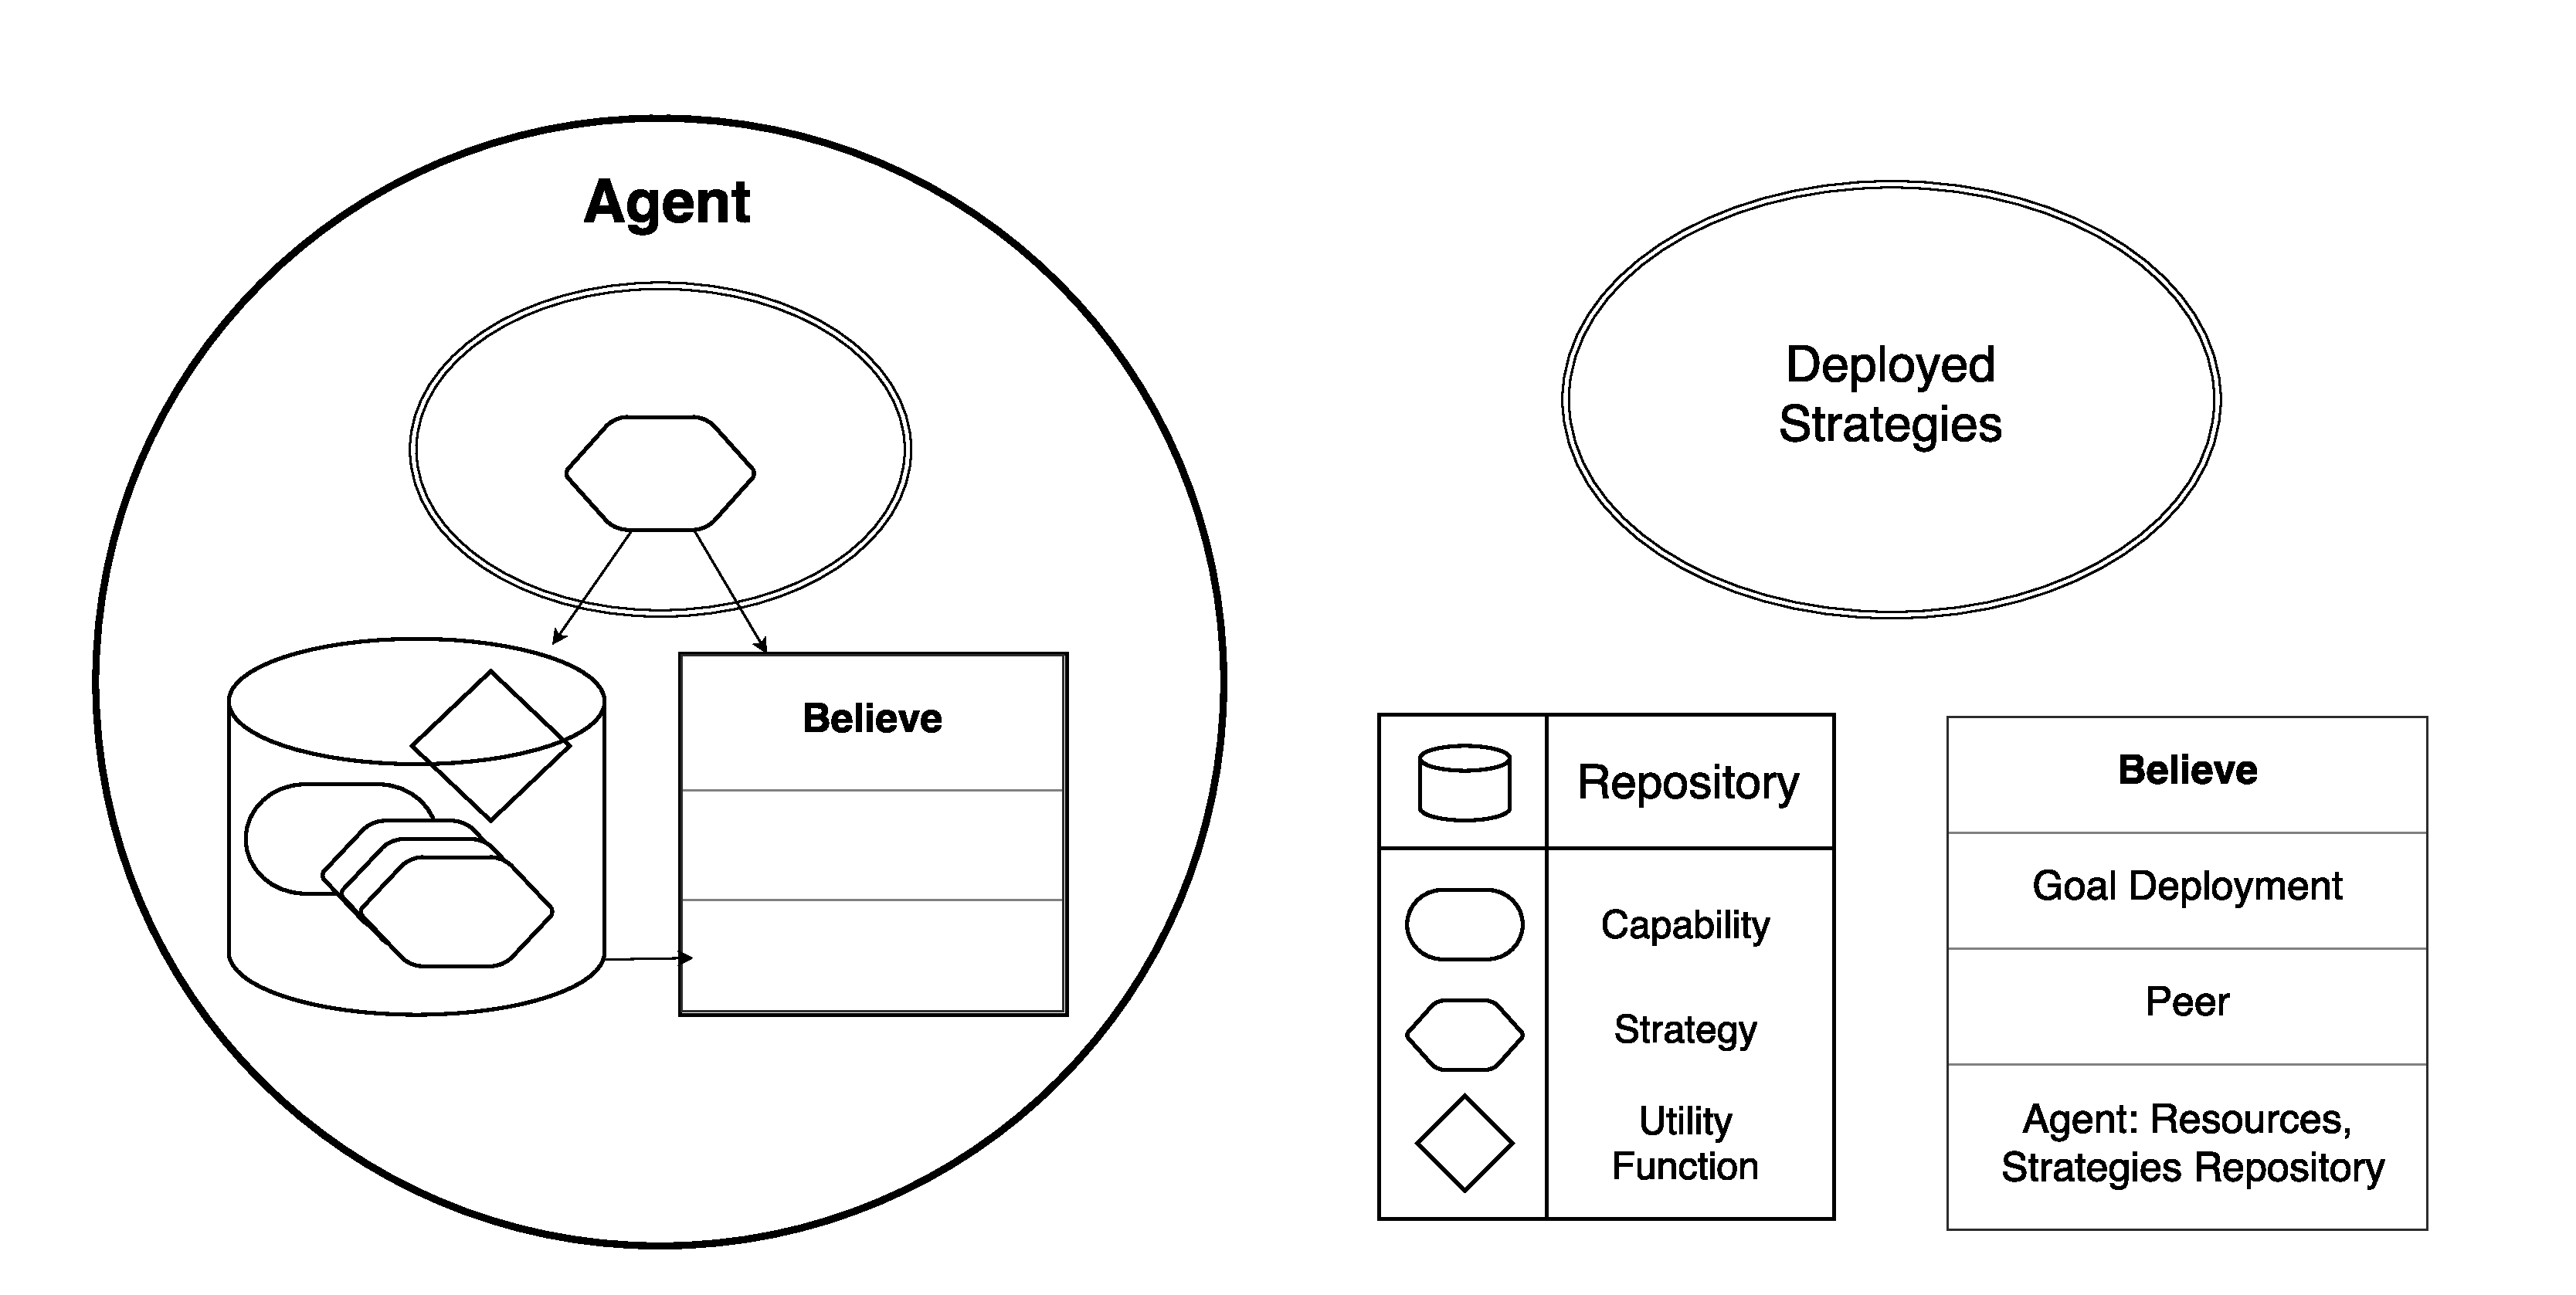
\includegraphics[width=\linewidth]{goalp-agent-repo-rcm-depl}
  \caption{The proposed agent composition}
  \label{fig:agent_composition}
\end{figure}

We followed an approach with run-time goal model with an mechanism for compositional adaptation and multi-agent collaboration. In our propose adaptiveness is achieved by means of strategies matching an selection at runtime. For more flexibility we propose a symmetric design.

By composable simetry we mean that we should be able to compose strategies in new strategies, and made agents out of strategies and teams out of agents. All with the same interface, transparent for a peer client.
